\section{Bubble sort}
\label{sec:bubble_sort}

\begin{frame}
	\frametitle{Yesterday's experiment}
	
	\begin{center}
		\includegraphics[width=0.6\textwidth]{figures/experiment.jpg}\\
		\hspace*{15pt}\hbox{\scriptsize Image By:\thinspace{\itshape Stefan Hugtenburg}}
	\end{center}
\end{frame}

\begin{frame}
	\frametitle{Bubble sort}
	\framesubtitle{Getting rid of inversions}
	
	\begin{overlayarea}{\textwidth}{\textheight}
		\only<1>{
			\begin{questionblock}{Let's formalise}
				What did you do yesterday?
			\end{questionblock}
		}
		
			\pause
			\begin{answerblock}{Your algorithm}
				\begin{algorithmic}
					\While{$v_i > v_{i+1}$ for some $i$}
						\State Switch them around.	
					\EndWhile
				\end{algorithmic}
			\end{answerblock}
			\pause
			\begin{center}
			\begin{tikzpicture}[scale=0.85, transform shape]
	\only<3>{
		\foreach \x/\val in {0/1,1/20,2/42,3/22,4/17}{
			\node[draw,rectangle, fill=gray!10, minimum size =1cm] (c) at (\x,0) {\val};
		}
	}
	\only<4>{
		\foreach \x/\val/\col in {0/1/green,1/20/green,2/42/black,3/22/black,4/17/black}{
			\node[draw=\col,rectangle, fill=\col!10, minimum size =1cm] (c) at (\x,0) {\val};
		}
	}
	\only<5>{
		\foreach \x/\val/\col in {0/1/black,1/20/green,2/42/green,3/22/black,4/17/black}{
			\node[draw=\col,rectangle, fill=\col!10, minimum size =1cm] (c) at (\x,0) {\val};
		}
	}
	\only<6>{
		\foreach \x/\val/\col in {0/1/black,1/20/black,2/42/red,3/22/red,4/17/black}{
			\node[draw=\col,rectangle, fill=\col!10, minimum size =1cm] (c) at (\x,0) {\val};
		}
	}
	\only<7>{
		\foreach \x/\val/\col in {0/1/black,1/20/black,2/22/green,3/42/green,4/17/black}{
			\node[draw=\col,rectangle, fill=\col!10, minimum size =1cm] (c) at (\x,0) {\val};
		}
	}
	\only<8>{
		\foreach \x/\val/\col in {0/1/black,1/20/black,2/22/black,3/42/red,4/17/red}{
			\node[draw=\col,rectangle, fill=\col!10, minimum size =1cm] (c) at (\x,0) {\val};
		}
	}
	\only<9>{
		\foreach \x/\val/\col in {0/1/black,1/20/black,2/22/black,3/17/green,4/42/green}{
			\node[draw=\col,rectangle, fill=\col!10, minimum size =1cm] (c) at (\x,0) {\val};
		}
	}
	\only<10>{
		\foreach \x/\val/\col in {0/1/green,1/20/green,2/22/black,3/17/black,4/42/black}{
			\node[draw=\col,rectangle, fill=\col!10, minimum size =1cm] (c) at (\x,0) {\val};
		}
	}
	\only<11>{
		\foreach \x/\val/\col in {0/1/black,1/20/green,2/22/green,3/17/black,4/42/black}{
			\node[draw=\col,rectangle, fill=\col!10, minimum size =1cm] (c) at (\x,0) {\val};
		}
	}
	\only<12>{
		\foreach \x/\val/\col in {0/1/black,1/20/black,2/22/red,3/17/red,4/42/black}{
			\node[draw=\col,rectangle, fill=\col!10, minimum size =1cm] (c) at (\x,0) {\val};
		}
	}
	\only<13>{
		\foreach \x/\val/\col in {0/1/black,1/20/black,2/17/green,3/22/green,4/42/black}{
			\node[draw=\col,rectangle, fill=\col!10, minimum size =1cm] (c) at (\x,0) {\val};
		}
	}
	\only<14>{
		\foreach \x/\val/\col in {0/1/black,1/20/black,2/17/black,3/22/green,4/42/green}{
			\node[draw=\col,rectangle, fill=\col!10, minimum size =1cm] (c) at (\x,0) {\val};
		}
	}
	\only<15>{
		\foreach \x/\val/\col in {0/1/green,1/20/green,2/17/black,3/22/black,4/42/black}{
			\node[draw=\col,rectangle, fill=\col!10, minimum size =1cm] (c) at (\x,0) {\val};
		}
	}
	\only<16>{
		\foreach \x/\val/\col in {0/1/black,1/20/red,2/17/red,3/22/black,4/42/black}{
			\node[draw=\col,rectangle, fill=\col!10, minimum size =1cm] (c) at (\x,0) {\val};
		}
	}
	\only<17>{
		\foreach \x/\val/\col in {0/1/black,1/17/green,2/20/green,3/22/black,4/42/black}{
			\node[draw=\col,rectangle, fill=\col!10, minimum size =1cm] (c) at (\x,0) {\val};
		}
	}
	\only<18>{
		\foreach \x/\val/\col in {0/1/black,1/17/black,2/20/green,3/22/green,4/42/black}{
			\node[draw=\col,rectangle, fill=\col!10, minimum size =1cm] (c) at (\x,0) {\val};
		}
	}
	\only<19>{
		\foreach \x/\val/\col in {0/1/black,1/17/black,2/20/black,3/22/green,4/42/green}{
			\node[draw=\col,rectangle, fill=\col!10, minimum size =1cm] (c) at (\x,0) {\val};
		}
	}
	\only<20>{
		\foreach \x/\val/\col in {0/1/green,1/17/green,2/20/black,3/22/black,4/42/black}{
			\node[draw=\col,rectangle, fill=\col!10, minimum size =1cm] (c) at (\x,0) {\val};
		}
	}
	\only<21>{
		\foreach \x/\val/\col in {0/1/black,1/17/green,2/20/green,3/22/black,4/42/black}{
			\node[draw=\col,rectangle, fill=\col!10, minimum size =1cm] (c) at (\x,0) {\val};
		}
	}
	\only<22>{
		\foreach \x/\val/\col in {0/1/black,1/17/black,2/20/green,3/22/green,4/42/black}{
			\node[draw=\col,rectangle, fill=\col!10, minimum size =1cm] (c) at (\x,0) {\val};
		}
	}
	\only<23->{
		\foreach \x/\val/\col in {0/1/black,1/17/black,2/20/black,3/22/green,4/42/green}{
			\node[draw=\col,rectangle, fill=\col!10, minimum size =1cm] (c) at (\x,0) {\val};
		}
	}
\end{tikzpicture}

			\end{center}
			\only<24->{
			\begin{questionblock}{Sounds easy...}
				So how many inversions can there be?
				\begin{multicols}{2}
				\begin{enumerate}[A.]
					\item $\Theta(n)$
					\item $\Theta(n^2)$
					\item $\Theta(n^n)$
					\item $\Theta(n!)$
				\end{enumerate}
			\end{multicols}
			\end{questionblock}
		}
	\end{overlayarea}
\end{frame}

\begin{frame}
	\frametitle{The number of inversions}
	\framesubtitle{What is the worst-case?}

	\begin{answerblock}{A list in reverse order}
		Remember yesterday? The people that were at the wrong end took the longest!\\
		\pause
		Consider a list in reverse order:
		\begin{itemize}
			\item The first element is wrong compared to all others: $n-1$ inversions.
		\pause
			\item The second is also wrong with all the ones that come after it: $n-2$ extra inversions.
			\item ...
		\pause
			\item The one-but last one is also wrong with the last one: $1$ inversion
		\pause
			\item So $\Theta(n^2)$ inversion!
		\end{itemize}
	\end{answerblock}
\end{frame}

\begin{frame}
	\frametitle{To summarise in code}
	\begin{columns}
		\column{0.565\textwidth}
	\lstinputlisting{code/bs.py}
		\column{0.455\textwidth}
		\begin{questionblock}{Pros and Cons?}
			What are the pros and cons of bubblesort? Hint: remember I told you it was slow!
		\end{questionblock}
	\end{columns}
\end{frame}

\begin{frame}
	\frametitle{Bubblesort: Pros and Cons}

		\begin{block}{Bubblesort}
			While there are inversions: fix them.
		\end{block}	
		\begin{exampleblock}{Pros}
			\begin{itemize}
				\item Great in a distributed setting, with autonomous agents (like students in a lecture hall).
				\item When implemented as: ``continue while there are inversion'' can terminate after one iteration over a
					sorted list! 
				\item Easiest to implement.
			\end{itemize}
		\end{exampleblock}	
		\begin{alertblock}{Cons}
			\begin{itemize}
				\item Terribly slow! (Often still slower than other $\Theta(n^2)$ algorithms we will see later)
			\end{itemize}
		\end{alertblock}	
\end{frame}
